\documentclass[1p]{elsarticle_modified}
%\bibliographystyle{elsarticle-num}

%\usepackage[colorlinks]{hyperref}
%\usepackage{abbrmath_seonhwa} %\Abb, \Ascr, \Acal ,\Abf, \Afrak
\usepackage{amsfonts}
\usepackage{amssymb}
\usepackage{amsmath}
\usepackage{amsthm}
\usepackage{scalefnt}
\usepackage{amsbsy}
\usepackage{kotex}
\usepackage{caption}
\usepackage{subfig}
\usepackage{color}
\usepackage{graphicx}
\usepackage{xcolor} %% white, black, red, green, blue, cyan, magenta, yellow
\usepackage{float}
\usepackage{setspace}
\usepackage{hyperref}

\usepackage{tikz}
\usetikzlibrary{arrows}

\usepackage{multirow}
\usepackage{array} % fixed length table
\usepackage{hhline}

%%%%%%%%%%%%%%%%%%%%%
\makeatletter
\renewcommand*\env@matrix[1][\arraystretch]{%
	\edef\arraystretch{#1}%
	\hskip -\arraycolsep
	\let\@ifnextchar\new@ifnextchar
	\array{*\c@MaxMatrixCols c}}
\makeatother %https://tex.stackexchange.com/questions/14071/how-can-i-increase-the-line-spacing-in-a-matrix
%%%%%%%%%%%%%%%

\usepackage[normalem]{ulem}

\newcommand{\msout}[1]{\ifmmode\text{\sout{\ensuremath{#1}}}\else\sout{#1}\fi}
%SOURCE: \msout is \stkout macro in https://tex.stackexchange.com/questions/20609/strikeout-in-math-mode

\newcommand{\cancel}[1]{
	\ifmmode
	{\color{red}\msout{#1}}
	\else
	{\color{red}\sout{#1}}
	\fi
}

\newcommand{\add}[1]{
	{\color{blue}\uwave{#1}}
}

\newcommand{\replace}[2]{
	\ifmmode
	{\color{red}\msout{#1}}{\color{blue}\uwave{#2}}
	\else
	{\color{red}\sout{#1}}{\color{blue}\uwave{#2}}
	\fi
}

\newcommand{\Sol}{\mathcal{S}} %segment
\newcommand{\D}{D} %diagram
\newcommand{\A}{\mathcal{A}} %arc


%%%%%%%%%%%%%%%%%%%%%%%%%%%%%5 test

\def\sl{\operatorname{\textup{SL}}(2,\Cbb)}
\def\psl{\operatorname{\textup{PSL}}(2,\Cbb)}
\def\quan{\mkern 1mu \triangleright \mkern 1mu}

\theoremstyle{definition}
\newtheorem{thm}{Theorem}[section]
\newtheorem{prop}[thm]{Proposition}
\newtheorem{lem}[thm]{Lemma}
\newtheorem{ques}[thm]{Question}
\newtheorem{cor}[thm]{Corollary}
\newtheorem{defn}[thm]{Definition}
\newtheorem{exam}[thm]{Example}
\newtheorem{rmk}[thm]{Remark}
\newtheorem{alg}[thm]{Algorithm}

\newcommand{\I}{\sqrt{-1}}
\begin{document}

%\begin{frontmatter}
%
%\title{Boundary parabolic representations of knots up to 8 crossings}
%
%%% Group authors per affiliation:
%\author{Yunhi Cho} 
%\address{Department of Mathematics, University of Seoul, Seoul, Korea}
%\ead{yhcho@uos.ac.kr}
%
%
%\author{Seonhwa Kim} %\fnref{s_kim}}
%\address{Center for Geometry and Physics, Institute for Basic Science, Pohang, 37673, Korea}
%\ead{ryeona17@ibs.re.kr}
%
%\author{Hyuk Kim}
%\address{Department of Mathematical Sciences, Seoul National University, Seoul 08826, Korea}
%\ead{hyukkim@snu.ac.kr}
%
%\author{Seokbeom Yoon}
%\address{Department of Mathematical Sciences, Seoul National University, Seoul, 08826,  Korea}
%\ead{sbyoon15@snu.ac.kr}
%
%\begin{abstract}
%We find all boundary parabolic representation of knots up to 8 crossings.
%
%\end{abstract}
%\begin{keyword}
%    \MSC[2010] 57M25 
%\end{keyword}
%
%\end{frontmatter}

%\linenumbers
%\tableofcontents
%
\newcommand\colored[1]{\textcolor{white}{\rule[-0.35ex]{0.8em}{1.4ex}}\kern-0.8em\color{red} #1}%
%\newcommand\colored[1]{\textcolor{white}{ #1}\kern-2.17ex	\textcolor{white}{ #1}\kern-1.81ex	\textcolor{white}{ #1}\kern-2.15ex\color{red}#1	}

{\Large $\underline{12n_{0050}~(K12n_{0050})}$}

\setlength{\tabcolsep}{10pt}
\renewcommand{\arraystretch}{1.6}
\vspace{1cm}\begin{tabular}{m{100pt}>{\centering\arraybackslash}m{274pt}}
\multirow{5}{120pt}{
	\centering
	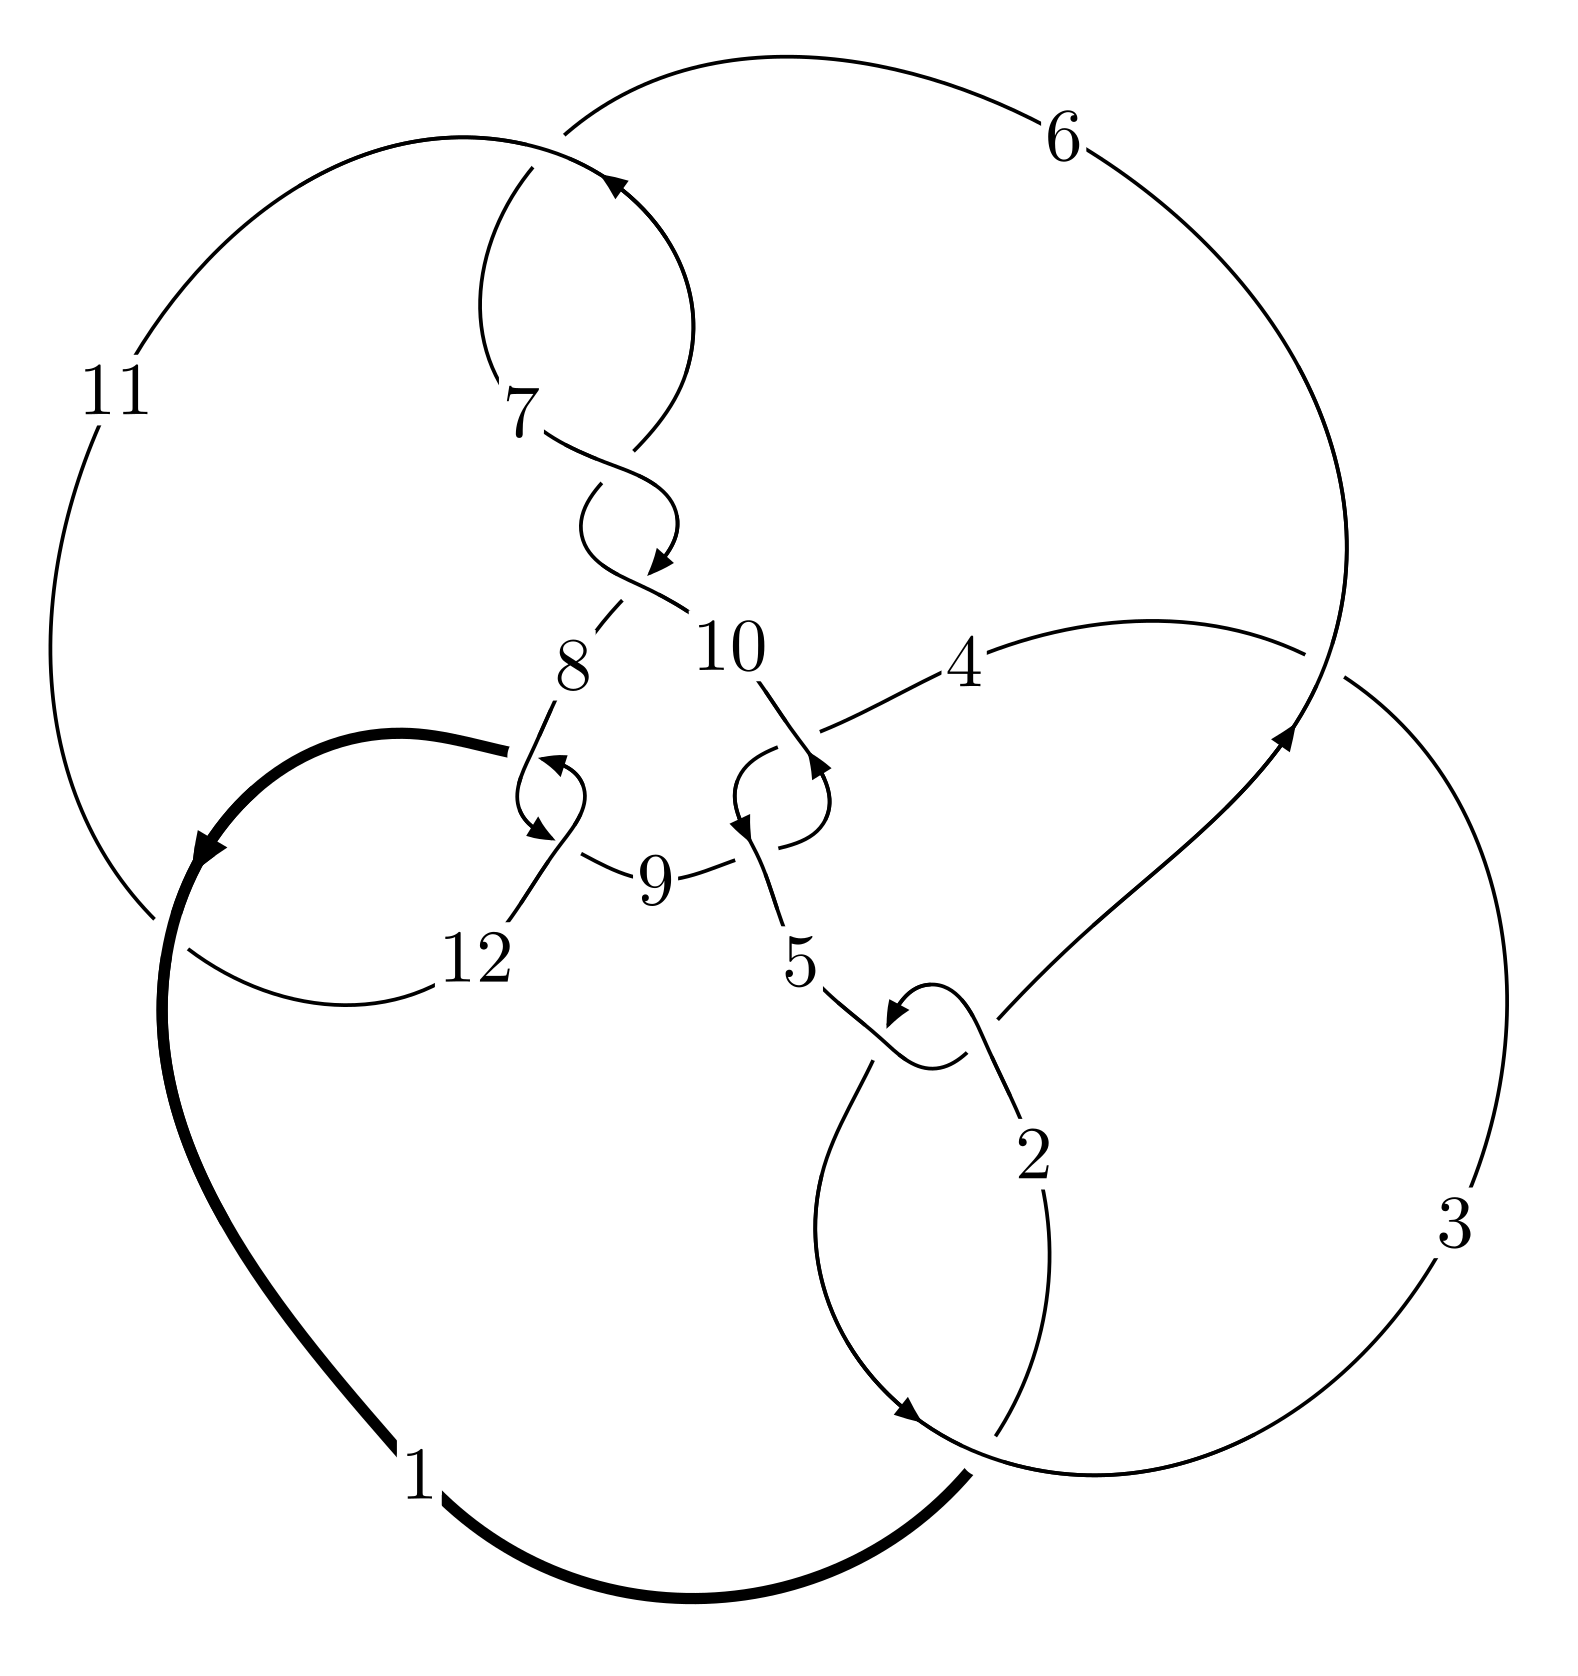
\includegraphics[width=112pt]{../../../GIT/diagram.site/Diagrams/png/2139_12n_0050.png}\\
\ \ \ A knot diagram\footnotemark}&
\allowdisplaybreaks
\textbf{Linearized knot diagam} \\
\cline{2-2}
 &
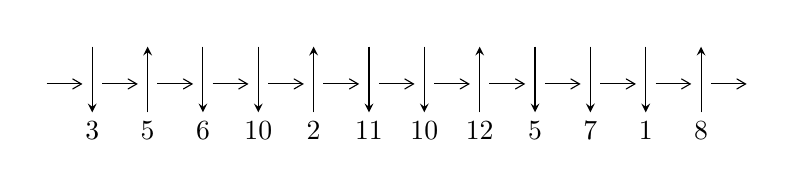
\begin{tikzpicture}[x=20pt, y=17pt]
	% nodes
	\node (C0) at (0, 0) {};
	\node (C1) at (1, 0) {};
	\node (C1U) at (1, +1) {};
	\node (C1D) at (1, -1) {3};

	\node (C2) at (2, 0) {};
	\node (C2U) at (2, +1) {};
	\node (C2D) at (2, -1) {5};

	\node (C3) at (3, 0) {};
	\node (C3U) at (3, +1) {};
	\node (C3D) at (3, -1) {6};

	\node (C4) at (4, 0) {};
	\node (C4U) at (4, +1) {};
	\node (C4D) at (4, -1) {10};

	\node (C5) at (5, 0) {};
	\node (C5U) at (5, +1) {};
	\node (C5D) at (5, -1) {2};

	\node (C6) at (6, 0) {};
	\node (C6U) at (6, +1) {};
	\node (C6D) at (6, -1) {11};

	\node (C7) at (7, 0) {};
	\node (C7U) at (7, +1) {};
	\node (C7D) at (7, -1) {10};

	\node (C8) at (8, 0) {};
	\node (C8U) at (8, +1) {};
	\node (C8D) at (8, -1) {12};

	\node (C9) at (9, 0) {};
	\node (C9U) at (9, +1) {};
	\node (C9D) at (9, -1) {5};

	\node (C10) at (10, 0) {};
	\node (C10U) at (10, +1) {};
	\node (C10D) at (10, -1) {7};

	\node (C11) at (11, 0) {};
	\node (C11U) at (11, +1) {};
	\node (C11D) at (11, -1) {1};

	\node (C12) at (12, 0) {};
	\node (C12U) at (12, +1) {};
	\node (C12D) at (12, -1) {8};
	\node (C13) at (13, 0) {};

	% arrows
	\draw[->,>={angle 60}]
	(C0) edge (C1) (C1) edge (C2) (C2) edge (C3) (C3) edge (C4) (C4) edge (C5) (C5) edge (C6) (C6) edge (C7) (C7) edge (C8) (C8) edge (C9) (C9) edge (C10) (C10) edge (C11) (C11) edge (C12) (C12) edge (C13) ;	\draw[->,>=stealth]
	(C1U) edge (C1D) (C2D) edge (C2U) (C3U) edge (C3D) (C4U) edge (C4D) (C5D) edge (C5U) (C6U) edge (C6D) (C7U) edge (C7D) (C8D) edge (C8U) (C9U) edge (C9D) (C10U) edge (C10D) (C11U) edge (C11D) (C12D) edge (C12U) ;
	\end{tikzpicture} \\
\hhline{~~} \\& 
\textbf{Solving Sequence} \\ \cline{2-2} 
 &
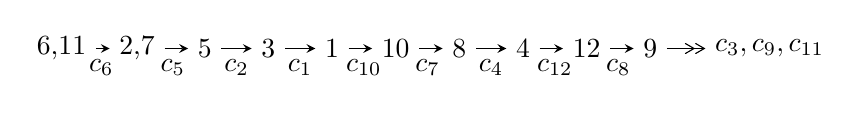
\begin{tikzpicture}[x=23pt, y=7pt]
	% node
	\node (A0) at (-1/8, 0) {6,11};
	\node (A1) at (17/16, 0) {2,7};
	\node (A2) at (17/8, 0) {5};
	\node (A3) at (25/8, 0) {3};
	\node (A4) at (33/8, 0) {1};
	\node (A5) at (41/8, 0) {10};
	\node (A6) at (49/8, 0) {8};
	\node (A7) at (57/8, 0) {4};
	\node (A8) at (65/8, 0) {12};
	\node (A9) at (73/8, 0) {9};
	\node (C1) at (1/2, -1) {$c_{6}$};
	\node (C2) at (13/8, -1) {$c_{5}$};
	\node (C3) at (21/8, -1) {$c_{2}$};
	\node (C4) at (29/8, -1) {$c_{1}$};
	\node (C5) at (37/8, -1) {$c_{10}$};
	\node (C6) at (45/8, -1) {$c_{7}$};
	\node (C7) at (53/8, -1) {$c_{4}$};
	\node (C8) at (61/8, -1) {$c_{12}$};
	\node (C9) at (69/8, -1) {$c_{8}$};
	\node (A10) at (11, 0) {$c_{3},c_{9},c_{11}$};

	% edge
	\draw[->,>=stealth]	
	(A0) edge (A1) (A1) edge (A2) (A2) edge (A3) (A3) edge (A4) (A4) edge (A5) (A5) edge (A6) (A6) edge (A7) (A7) edge (A8) (A8) edge (A9) ;
	\draw[->>,>={angle 60}]	
	(A9) edge (A10);
\end{tikzpicture} \\ 

\end{tabular} \\

\footnotetext{
The image of knot diagram is generated by the software ``\textbf{Draw programme}" developed by Andrew Bartholomew(\url{http://www.layer8.co.uk/maths/draw/index.htm\#Running-draw}), where we modified some parts for our purpose(\url{https://github.com/CATsTAILs/LinksPainter}).
}\phantom \\ \newline 
\centering \textbf{Ideals for irreducible components\footnotemark of $X_{\text{par}}$} 
 
\begin{align*}
I^u_{1}&=\langle 
1.86448\times10^{23} u^{41}-4.54607\times10^{23} u^{40}+\cdots+2.14051\times10^{24} b-1.33994\times10^{24},\\
\phantom{I^u_{1}}&\phantom{= \langle  }1.55777\times10^{24} u^{41}-3.49226\times10^{24} u^{40}+\cdots+4.28103\times10^{24} a-8.66921\times10^{24},\;u^{42}-3 u^{41}+\cdots-4 u+1\rangle \\
I^u_{2}&=\langle 
u^2 a- a u+u^2+b- u,\;2 u^3 a-4 u^2 a-5 u^3+4 a^2+6 a u+6 u^2-2 a-13 u+15,\;u^4- u^3+3 u^2-2 u+1\rangle \\
I^u_{3}&=\langle 
- u^6-2 u^4-2 u^3- u^2+b-2 u,\;- u^6-3 u^4-2 u^3-2 u^2+a-4 u-1,\\
\phantom{I^u_{3}}&\phantom{= \langle  }u^{15}+5 u^{13}+5 u^{12}+10 u^{11}+20 u^{10}+18 u^9+30 u^8+29 u^7+23 u^6+25 u^5+11 u^4+7 u^3+3 u^2- u+1\rangle \\
\\
\end{align*}
\raggedright * 3 irreducible components of $\dim_{\mathbb{C}}=0$, with total 65 representations.\\
\footnotetext{All coefficients of polynomials are rational numbers. But the coefficients are sometimes approximated in decimal forms when there is not enough margin.}
\newpage
\renewcommand{\arraystretch}{1}
\centering \section*{I. $I^u_{1}= \langle 1.86\times10^{23} u^{41}-4.55\times10^{23} u^{40}+\cdots+2.14\times10^{24} b-1.34\times10^{24},\;1.56\times10^{24} u^{41}-3.49\times10^{24} u^{40}+\cdots+4.28\times10^{24} a-8.67\times10^{24},\;u^{42}-3 u^{41}+\cdots-4 u+1 \rangle$}
\flushleft \textbf{(i) Arc colorings}\\
\begin{tabular}{m{7pt} m{180pt} m{7pt} m{180pt} }
\flushright $a_{6}=$&$\begin{pmatrix}1\\0\end{pmatrix}$ \\
\flushright $a_{11}=$&$\begin{pmatrix}0\\u\end{pmatrix}$ \\
\flushright $a_{2}=$&$\begin{pmatrix}-0.363877 u^{41}+0.815753 u^{40}+\cdots-0.334201 u+2.02503\\-0.0871043 u^{41}+0.212382 u^{40}+\cdots-0.482611 u+0.625989\end{pmatrix}$ \\
\flushright $a_{7}=$&$\begin{pmatrix}1\\u^2\end{pmatrix}$ \\
\flushright $a_{5}=$&$\begin{pmatrix}-0.659564 u^{41}+1.39975 u^{40}+\cdots+0.0845241 u+0.435332\\-0.0702325 u^{41}+0.143960 u^{40}+\cdots-0.391861 u-0.363693\end{pmatrix}$ \\
\flushright $a_{3}=$&$\begin{pmatrix}-0.574443 u^{41}+1.03501 u^{40}+\cdots+1.04901 u-0.509224\\0.0313582 u^{41}-0.169378 u^{40}+\cdots+0.191274 u-0.637085\end{pmatrix}$ \\
\flushright $a_{1}=$&$\begin{pmatrix}0.545703 u^{41}-1.87495 u^{40}+\cdots+6.14055 u-3.12407\\0.0705453 u^{41}-0.437164 u^{40}+\cdots+2.10999 u-0.698937\end{pmatrix}$ \\
\flushright $a_{10}=$&$\begin{pmatrix}u\\u^3+u\end{pmatrix}$ \\
\flushright $a_{8}=$&$\begin{pmatrix}u^2+1\\u^4+2 u^2\end{pmatrix}$ \\
\flushright $a_{4}=$&$\begin{pmatrix}-0.605801 u^{41}+1.20439 u^{40}+\cdots+0.857736 u+0.127861\\0.0313582 u^{41}-0.169378 u^{40}+\cdots+0.191274 u-0.637085\end{pmatrix}$ \\
\flushright $a_{12}=$&$\begin{pmatrix}0.112025 u^{41}-0.738600 u^{40}+\cdots+1.78402 u-2.01029\\-0.179156 u^{41}+0.123997 u^{40}+\cdots+1.38787 u-0.296413\end{pmatrix}$ \\
\flushright $a_{9}=$&$\begin{pmatrix}0.711251 u^{41}-1.94978 u^{40}+\cdots+4.85792 u-0.210599\\-0.0109483 u^{41}+0.102515 u^{40}+\cdots+0.549153 u+0.291182\end{pmatrix}$\\&\end{tabular}
\flushleft \textbf{(ii) Obstruction class $= -1$}\\~\\
\flushleft \textbf{(iii) Cusp Shapes $= \frac{8819869146154630149250287}{8562054330498891123064064} u^{41}-\frac{6951105346810345728611581}{2140513582624722780766016} u^{40}+\cdots-\frac{9809601898657334062772699}{8562054330498891123064064} u-\frac{77878813575983057100937417}{8562054330498891123064064}$}\\~\\
\newpage\renewcommand{\arraystretch}{1}
\flushleft \textbf{(iv) u-Polynomials at the component}\newline \\
\begin{tabular}{m{50pt}|m{274pt}}
Crossings & \hspace{64pt}u-Polynomials at each crossing \\
\hline $$\begin{aligned}c_{1}\end{aligned}$$&$\begin{aligned}
&u^{42}+22 u^{41}+\cdots+383 u+16
\end{aligned}$\\
\hline $$\begin{aligned}c_{2},c_{5}\end{aligned}$$&$\begin{aligned}
&u^{42}+2 u^{41}+\cdots-3 u+4
\end{aligned}$\\
\hline $$\begin{aligned}c_{3}\end{aligned}$$&$\begin{aligned}
&u^{42}-2 u^{41}+\cdots-23400 u+3104
\end{aligned}$\\
\hline $$\begin{aligned}c_{4},c_{9}\end{aligned}$$&$\begin{aligned}
&u^{42}+2 u^{41}+\cdots+3584 u+2048
\end{aligned}$\\
\hline $$\begin{aligned}c_{6},c_{7},c_{10}\end{aligned}$$&$\begin{aligned}
&u^{42}-3 u^{41}+\cdots-4 u+1
\end{aligned}$\\
\hline $$\begin{aligned}c_{8},c_{12}\end{aligned}$$&$\begin{aligned}
&u^{42}-3 u^{41}+\cdots-2 u+1
\end{aligned}$\\
\hline $$\begin{aligned}c_{11}\end{aligned}$$&$\begin{aligned}
&u^{42}+23 u^{41}+\cdots+6 u+1
\end{aligned}$\\
\hline
\end{tabular}\\~\\
\newpage\renewcommand{\arraystretch}{1}
\flushleft \textbf{(v) Riley Polynomials at the component}\newline \\
\begin{tabular}{m{50pt}|m{274pt}}
Crossings & \hspace{64pt}Riley Polynomials at each crossing \\
\hline $$\begin{aligned}c_{1}\end{aligned}$$&$\begin{aligned}
&y^{42}-2 y^{41}+\cdots+33759 y+256
\end{aligned}$\\
\hline $$\begin{aligned}c_{2},c_{5}\end{aligned}$$&$\begin{aligned}
&y^{42}+22 y^{41}+\cdots+383 y+16
\end{aligned}$\\
\hline $$\begin{aligned}c_{3}\end{aligned}$$&$\begin{aligned}
&y^{42}-26 y^{41}+\cdots+359975104 y+9634816
\end{aligned}$\\
\hline $$\begin{aligned}c_{4},c_{9}\end{aligned}$$&$\begin{aligned}
&y^{42}-30 y^{41}+\cdots-36438016 y+4194304
\end{aligned}$\\
\hline $$\begin{aligned}c_{6},c_{7},c_{10}\end{aligned}$$&$\begin{aligned}
&y^{42}+35 y^{41}+\cdots+6 y+1
\end{aligned}$\\
\hline $$\begin{aligned}c_{8},c_{12}\end{aligned}$$&$\begin{aligned}
&y^{42}+23 y^{41}+\cdots+6 y+1
\end{aligned}$\\
\hline $$\begin{aligned}c_{11}\end{aligned}$$&$\begin{aligned}
&y^{42}-5 y^{41}+\cdots-54 y+1
\end{aligned}$\\
\hline
\end{tabular}\\~\\
\newpage\flushleft \textbf{(vi) Complex Volumes and Cusp Shapes}
$$\begin{array}{c|c|c}  
\text{Solutions to }I^u_{1}& \I (\text{vol} + \sqrt{-1}CS) & \text{Cusp shape}\\
 \hline 
\begin{aligned}
u &= \phantom{-}1.027970 + 0.100105 I \\
a &= \phantom{-}0.24960 + 1.85629 I \\
b &= -0.546190 + 1.233220 I\end{aligned}
 & -9.37503 - 10.09150 I & -8.44713 + 6.42657 I \\ \hline\begin{aligned}
u &= \phantom{-}1.027970 - 0.100105 I \\
a &= \phantom{-}0.24960 - 1.85629 I \\
b &= -0.546190 - 1.233220 I\end{aligned}
 & -9.37503 + 10.09150 I & -8.44713 - 6.42657 I \\ \hline\begin{aligned}
u &= \phantom{-}0.929724 + 0.138462 I \\
a &= \phantom{-}0.54776 + 2.00727 I \\
b &= -0.357906 + 1.293250 I\end{aligned}
 & -10.74190 + 0.44052 I & -10.40215 + 0.18999 I \\ \hline\begin{aligned}
u &= \phantom{-}0.929724 - 0.138462 I \\
a &= \phantom{-}0.54776 - 2.00727 I \\
b &= -0.357906 - 1.293250 I\end{aligned}
 & -10.74190 - 0.44052 I & -10.40215 - 0.18999 I \\ \hline\begin{aligned}
u &= \phantom{-}0.914941 + 0.045259 I \\
a &= -0.416878 - 0.222543 I \\
b &= -0.915244 - 0.158700 I\end{aligned}
 & -6.11647 - 4.80305 I & -6.31453 + 3.22976 I \\ \hline\begin{aligned}
u &= \phantom{-}0.914941 - 0.045259 I \\
a &= -0.416878 + 0.222543 I \\
b &= -0.915244 + 0.158700 I\end{aligned}
 & -6.11647 + 4.80305 I & -6.31453 - 3.22976 I \\ \hline\begin{aligned}
u &= \phantom{-}0.176790 + 1.089910 I \\
a &= -1.33651 - 1.33318 I \\
b &= \phantom{-}0.552991 - 1.072730 I\end{aligned}
 & \phantom{-}1.83107 - 3.60410 I & \phantom{-}1.23384 + 2.84738 I \\ \hline\begin{aligned}
u &= \phantom{-}0.176790 - 1.089910 I \\
a &= -1.33651 + 1.33318 I \\
b &= \phantom{-}0.552991 + 1.072730 I\end{aligned}
 & \phantom{-}1.83107 + 3.60410 I & \phantom{-}1.23384 - 2.84738 I \\ \hline\begin{aligned}
u &= -0.638546 + 0.536386 I \\
a &= \phantom{-}1.17338 - 1.37011 I \\
b &= -0.089750 - 0.808861 I\end{aligned}
 & -1.04750 + 2.07664 I & -7.01132 - 2.89392 I \\ \hline\begin{aligned}
u &= -0.638546 - 0.536386 I \\
a &= \phantom{-}1.17338 + 1.37011 I \\
b &= -0.089750 + 0.808861 I\end{aligned}
 & -1.04750 - 2.07664 I & -7.01132 + 2.89392 I\\
 \hline 
 \end{array}$$\newpage$$\begin{array}{c|c|c}  
\text{Solutions to }I^u_{1}& \I (\text{vol} + \sqrt{-1}CS) & \text{Cusp shape}\\
 \hline 
\begin{aligned}
u &= -0.257246 + 1.141800 I \\
a &= -0.74697 + 1.25063 I \\
b &= \phantom{-}0.48378 + 1.32908 I\end{aligned}
 & -0.81918 + 6.49392 I & -4.00000 - 8.90623 I \\ \hline\begin{aligned}
u &= -0.257246 - 1.141800 I \\
a &= -0.74697 - 1.25063 I \\
b &= \phantom{-}0.48378 - 1.32908 I\end{aligned}
 & -0.81918 - 6.49392 I & -4.00000 + 8.90623 I \\ \hline\begin{aligned}
u &= -0.051623 + 1.181420 I \\
a &= -0.529834 - 0.226212 I \\
b &= \phantom{-}0.820994 + 0.618988 I\end{aligned}
 & \phantom{-}3.71536 + 1.69010 I & \phantom{-}3.26218 - 1.55976 I \\ \hline\begin{aligned}
u &= -0.051623 - 1.181420 I \\
a &= -0.529834 + 0.226212 I \\
b &= \phantom{-}0.820994 - 0.618988 I\end{aligned}
 & \phantom{-}3.71536 - 1.69010 I & \phantom{-}3.26218 + 1.55976 I \\ \hline\begin{aligned}
u &= \phantom{-}0.118844 + 1.181270 I \\
a &= -0.851838 - 0.430624 I \\
b &= \phantom{-}0.891940 - 0.979743 I\end{aligned}
 & \phantom{-}2.63448 - 4.63960 I & \phantom{-0.000000 -}0. + 8.16254 I \\ \hline\begin{aligned}
u &= \phantom{-}0.118844 - 1.181270 I \\
a &= -0.851838 + 0.430624 I \\
b &= \phantom{-}0.891940 + 0.979743 I\end{aligned}
 & \phantom{-}2.63448 + 4.63960 I & \phantom{-0.000000 } 0. - 8.16254 I \\ \hline\begin{aligned}
u &= -0.023170 + 1.204780 I \\
a &= -0.160324 - 0.092419 I \\
b &= \phantom{-}0.914501 + 0.286896 I\end{aligned}
 & \phantom{-}3.99481 + 1.55693 I & \phantom{-}4.40114 - 3.96530 I \\ \hline\begin{aligned}
u &= -0.023170 - 1.204780 I \\
a &= -0.160324 + 0.092419 I \\
b &= \phantom{-}0.914501 - 0.286896 I\end{aligned}
 & \phantom{-}3.99481 - 1.55693 I & \phantom{-}4.40114 + 3.96530 I \\ \hline\begin{aligned}
u &= \phantom{-}0.487771 + 1.186180 I \\
a &= -0.360345 - 1.006100 I \\
b &= -0.229714 - 1.369840 I\end{aligned}
 & -7.52698 - 5.48459 I & \phantom{-0.000000 } 0 \\ \hline\begin{aligned}
u &= \phantom{-}0.487771 - 1.186180 I \\
a &= -0.360345 + 1.006100 I \\
b &= -0.229714 + 1.369840 I\end{aligned}
 & -7.52698 + 5.48459 I & \phantom{-0.000000 } 0\\
 \hline 
 \end{array}$$\newpage$$\begin{array}{c|c|c}  
\text{Solutions to }I^u_{1}& \I (\text{vol} + \sqrt{-1}CS) & \text{Cusp shape}\\
 \hline 
\begin{aligned}
u &= -0.579810 + 1.160310 I \\
a &= -0.178403 + 0.945878 I \\
b &= -0.304232 + 1.178570 I\end{aligned}
 & -2.78929 + 1.17087 I & \phantom{-0.000000 } 0 \\ \hline\begin{aligned}
u &= -0.579810 - 1.160310 I \\
a &= -0.178403 - 0.945878 I \\
b &= -0.304232 - 1.178570 I\end{aligned}
 & -2.78929 - 1.17087 I & \phantom{-0.000000 } 0 \\ \hline\begin{aligned}
u &= -0.404098 + 1.316080 I \\
a &= \phantom{-}0.296578 - 0.436654 I \\
b &= -0.825719 + 0.274258 I\end{aligned}
 & \phantom{-}1.73633 + 4.52361 I & \phantom{-0.000000 } 0 \\ \hline\begin{aligned}
u &= -0.404098 - 1.316080 I \\
a &= \phantom{-}0.296578 + 0.436654 I \\
b &= -0.825719 - 0.274258 I\end{aligned}
 & \phantom{-}1.73633 - 4.52361 I & \phantom{-0.000000 } 0 \\ \hline\begin{aligned}
u &= \phantom{-}0.438573 + 1.326070 I \\
a &= \phantom{-}0.146351 + 0.500553 I \\
b &= -0.991101 - 0.284626 I\end{aligned}
 & -1.83637 - 9.65354 I & \phantom{-0.000000 } 0 \\ \hline\begin{aligned}
u &= \phantom{-}0.438573 - 1.326070 I \\
a &= \phantom{-}0.146351 - 0.500553 I \\
b &= -0.991101 + 0.284626 I\end{aligned}
 & -1.83637 + 9.65354 I & \phantom{-0.000000 } 0 \\ \hline\begin{aligned}
u &= \phantom{-}0.48276 + 1.38315 I \\
a &= \phantom{-}1.29723 + 1.22335 I \\
b &= -0.619520 + 1.226280 I\end{aligned}
 & -4.7316 - 15.4661 I & \phantom{-0.000000 } 0 \\ \hline\begin{aligned}
u &= \phantom{-}0.48276 - 1.38315 I \\
a &= \phantom{-}1.29723 - 1.22335 I \\
b &= -0.619520 - 1.226280 I\end{aligned}
 & -4.7316 + 15.4661 I & \phantom{-0.000000 } 0 \\ \hline\begin{aligned}
u &= -0.518309 + 0.081810 I \\
a &= \phantom{-}1.62251 - 2.04492 I \\
b &= \phantom{-}0.313840 - 1.152440 I\end{aligned}
 & -3.86435 - 3.51413 I & -10.49218 + 3.82170 I \\ \hline\begin{aligned}
u &= -0.518309 - 0.081810 I \\
a &= \phantom{-}1.62251 + 2.04492 I \\
b &= \phantom{-}0.313840 + 1.152440 I\end{aligned}
 & -3.86435 + 3.51413 I & -10.49218 - 3.82170 I\\
 \hline 
 \end{array}$$\newpage$$\begin{array}{c|c|c}  
\text{Solutions to }I^u_{1}& \I (\text{vol} + \sqrt{-1}CS) & \text{Cusp shape}\\
 \hline 
\begin{aligned}
u &= -0.46833 + 1.40959 I \\
a &= \phantom{-}1.28786 - 1.10744 I \\
b &= -0.562936 - 1.175720 I\end{aligned}
 & -0.96374 + 9.68671 I & \phantom{-0.000000 } 0 \\ \hline\begin{aligned}
u &= -0.46833 - 1.40959 I \\
a &= \phantom{-}1.28786 + 1.10744 I \\
b &= -0.562936 + 1.175720 I\end{aligned}
 & -0.96374 - 9.68671 I & \phantom{-0.000000 } 0 \\ \hline\begin{aligned}
u &= -0.256255 + 0.421847 I \\
a &= \phantom{-}1.193230 + 0.520583 I \\
b &= \phantom{-}0.123371 + 0.236807 I\end{aligned}
 & -0.427988 + 1.171450 I & -4.97387 - 5.79413 I \\ \hline\begin{aligned}
u &= -0.256255 - 0.421847 I \\
a &= \phantom{-}1.193230 - 0.520583 I \\
b &= \phantom{-}0.123371 - 0.236807 I\end{aligned}
 & -0.427988 - 1.171450 I & -4.97387 + 5.79413 I \\ \hline\begin{aligned}
u &= -0.05066 + 1.56885 I \\
a &= \phantom{-}0.821923 + 0.217869 I \\
b &= -0.377724 + 0.762011 I\end{aligned}
 & \phantom{-}6.69834 + 1.66397 I & \phantom{-0.000000 } 0 \\ \hline\begin{aligned}
u &= -0.05066 - 1.56885 I \\
a &= \phantom{-}0.821923 - 0.217869 I \\
b &= -0.377724 - 0.762011 I\end{aligned}
 & \phantom{-}6.69834 - 1.66397 I & \phantom{-0.000000 } 0 \\ \hline\begin{aligned}
u &= \phantom{-}0.040527 + 0.421390 I \\
a &= \phantom{-}2.04288 + 1.54331 I \\
b &= \phantom{-}0.455512 + 0.708227 I\end{aligned}
 & -0.32690 + 1.38361 I & -5.63624 - 5.27111 I \\ \hline\begin{aligned}
u &= \phantom{-}0.040527 - 0.421390 I \\
a &= \phantom{-}2.04288 - 1.54331 I \\
b &= \phantom{-}0.455512 - 0.708227 I\end{aligned}
 & -0.32690 - 1.38361 I & -5.63624 + 5.27111 I \\ \hline\begin{aligned}
u &= -0.14166 + 1.59539 I \\
a &= \phantom{-}1.013790 - 0.413700 I \\
b &= -0.360591 - 0.879206 I\end{aligned}
 & \phantom{-}6.34972 + 4.89959 I & \phantom{-0.000000 } 0 \\ \hline\begin{aligned}
u &= -0.14166 - 1.59539 I \\
a &= \phantom{-}1.013790 + 0.413700 I \\
b &= -0.360591 + 0.879206 I\end{aligned}
 & \phantom{-}6.34972 - 4.89959 I & \phantom{-0.000000 } 0\\
 \hline 
 \end{array}$$\newpage$$\begin{array}{c|c|c}  
\text{Solutions to }I^u_{1}& \I (\text{vol} + \sqrt{-1}CS) & \text{Cusp shape}\\
 \hline 
\begin{aligned}
u &= \phantom{-}0.271803 + 0.171548 I \\
a &= \phantom{-}2.13801 - 1.84885 I \\
b &= \phantom{-}0.623695 - 0.921062 I\end{aligned}
 & -1.06689 - 3.17946 I & -11.00684 + 2.84027 I \\ \hline\begin{aligned}
u &= \phantom{-}0.271803 - 0.171548 I \\
a &= \phantom{-}2.13801 + 1.84885 I \\
b &= \phantom{-}0.623695 + 0.921062 I\end{aligned}
 & -1.06689 + 3.17946 I & -11.00684 - 2.84027 I\\
 \hline 
 \end{array}$$\newpage\newpage\renewcommand{\arraystretch}{1}
\centering \section*{II. $I^u_{2}= \langle u^2 a- a u+u^2+b- u,\;2 u^3 a-5 u^3+\cdots-2 a+15,\;u^4- u^3+3 u^2-2 u+1 \rangle$}
\flushleft \textbf{(i) Arc colorings}\\
\begin{tabular}{m{7pt} m{180pt} m{7pt} m{180pt} }
\flushright $a_{6}=$&$\begin{pmatrix}1\\0\end{pmatrix}$ \\
\flushright $a_{11}=$&$\begin{pmatrix}0\\u\end{pmatrix}$ \\
\flushright $a_{2}=$&$\begin{pmatrix}a\\- u^2 a+a u- u^2+u\end{pmatrix}$ \\
\flushright $a_{7}=$&$\begin{pmatrix}1\\u^2\end{pmatrix}$ \\
\flushright $a_{5}=$&$\begin{pmatrix}u^2 a+\frac{1}{2} u^3- a u+a+\frac{1}{2} u-\frac{1}{2}\\- u^2 a+a u- u^2+u-1\end{pmatrix}$ \\
\flushright $a_{3}=$&$\begin{pmatrix}\frac{1}{2} u^3- u^2+a+\frac{3}{2} u-\frac{3}{2}\\- u^2 a+a u- u^2+u-1\end{pmatrix}$ \\
\flushright $a_{1}=$&$\begin{pmatrix}-1\\0\end{pmatrix}$ \\
\flushright $a_{10}=$&$\begin{pmatrix}u\\u^3+u\end{pmatrix}$ \\
\flushright $a_{8}=$&$\begin{pmatrix}u^2+1\\u^3- u^2+2 u-1\end{pmatrix}$ \\
\flushright $a_{4}=$&$\begin{pmatrix}u^2 a+\frac{1}{2} u^3- a u+a+\frac{1}{2} u-\frac{1}{2}\\- u^2 a+a u- u^2+u-1\end{pmatrix}$ \\
\flushright $a_{12}=$&$\begin{pmatrix}- u\\u\end{pmatrix}$ \\
\flushright $a_{9}=$&$\begin{pmatrix}u\\u^3+u\end{pmatrix}$\\&\end{tabular}
\flushleft \textbf{(ii) Obstruction class $= 1$}\\~\\
\flushleft \textbf{(iii) Cusp Shapes $= -\frac{3}{2} u^3 a+11 u^2 a+\frac{7}{2} u^3-\frac{15}{2} a u+5 u^2+\frac{5}{2} a+\frac{11}{2} u-\frac{7}{2}$}\\~\\
\newpage\renewcommand{\arraystretch}{1}
\flushleft \textbf{(iv) u-Polynomials at the component}\newline \\
\begin{tabular}{m{50pt}|m{274pt}}
Crossings & \hspace{64pt}u-Polynomials at each crossing \\
\hline $$\begin{aligned}c_{1},c_{3},c_{5}\end{aligned}$$&$\begin{aligned}
&(u^2- u+1)^4
\end{aligned}$\\
\hline $$\begin{aligned}c_{2}\end{aligned}$$&$\begin{aligned}
&(u^2+u+1)^4
\end{aligned}$\\
\hline $$\begin{aligned}c_{4},c_{9}\end{aligned}$$&$\begin{aligned}
&u^8
\end{aligned}$\\
\hline $$\begin{aligned}c_{6},c_{7},c_{11}\end{aligned}$$&$\begin{aligned}
&(u^4- u^3+3 u^2-2 u+1)^2
\end{aligned}$\\
\hline $$\begin{aligned}c_{8}\end{aligned}$$&$\begin{aligned}
&(u^4- u^3+u^2+1)^2
\end{aligned}$\\
\hline $$\begin{aligned}c_{10}\end{aligned}$$&$\begin{aligned}
&(u^4+u^3+3 u^2+2 u+1)^2
\end{aligned}$\\
\hline $$\begin{aligned}c_{12}\end{aligned}$$&$\begin{aligned}
&(u^4+u^3+u^2+1)^2
\end{aligned}$\\
\hline
\end{tabular}\\~\\
\newpage\renewcommand{\arraystretch}{1}
\flushleft \textbf{(v) Riley Polynomials at the component}\newline \\
\begin{tabular}{m{50pt}|m{274pt}}
Crossings & \hspace{64pt}Riley Polynomials at each crossing \\
\hline $$\begin{aligned}c_{1},c_{2},c_{3}\\c_{5}\end{aligned}$$&$\begin{aligned}
&(y^2+y+1)^4
\end{aligned}$\\
\hline $$\begin{aligned}c_{4},c_{9}\end{aligned}$$&$\begin{aligned}
&y^8
\end{aligned}$\\
\hline $$\begin{aligned}c_{6},c_{7},c_{10}\\c_{11}\end{aligned}$$&$\begin{aligned}
&(y^4+5 y^3+7 y^2+2 y+1)^2
\end{aligned}$\\
\hline $$\begin{aligned}c_{8},c_{12}\end{aligned}$$&$\begin{aligned}
&(y^4+y^3+3 y^2+2 y+1)^2
\end{aligned}$\\
\hline
\end{tabular}\\~\\
\newpage\flushleft \textbf{(vi) Complex Volumes and Cusp Shapes}
$$\begin{array}{c|c|c}  
\text{Solutions to }I^u_{2}& \I (\text{vol} + \sqrt{-1}CS) & \text{Cusp shape}\\
 \hline 
\begin{aligned}
u &= \phantom{-}0.395123 + 0.506844 I \\
a &= \phantom{-}0.32193 + 1.46300 I \\
b &= \phantom{-}0.500000 + 0.866025 I\end{aligned}
 & -0.211005 + 0.614778 I & -3.71851 + 3.54153 I \\ \hline\begin{aligned}
u &= \phantom{-}0.395123 + 0.506844 I \\
a &= -0.39397 - 1.87632 I \\
b &= \phantom{-}0.500000 - 0.866025 I\end{aligned}
 & -0.21101 - 3.44499 I & -1.37216 + 7.25656 I \\ \hline\begin{aligned}
u &= \phantom{-}0.395123 - 0.506844 I \\
a &= \phantom{-}0.32193 - 1.46300 I \\
b &= \phantom{-}0.500000 - 0.866025 I\end{aligned}
 & -0.211005 - 0.614778 I & -3.71851 - 3.54153 I \\ \hline\begin{aligned}
u &= \phantom{-}0.395123 - 0.506844 I \\
a &= -0.39397 + 1.87632 I \\
b &= \phantom{-}0.500000 + 0.866025 I\end{aligned}
 & -0.21101 + 3.44499 I & -1.37216 - 7.25656 I \\ \hline\begin{aligned}
u &= \phantom{-}0.10488 + 1.55249 I \\
a &= -0.975620 - 0.357786 I \\
b &= \phantom{-}0.500000 - 0.866025 I\end{aligned}
 & \phantom{-}6.79074 - 5.19385 I & \phantom{-}4.49529 + 8.13693 I \\ \hline\begin{aligned}
u &= \phantom{-}0.10488 + 1.55249 I \\
a &= -0.702338 + 0.200007 I \\
b &= \phantom{-}0.500000 + 0.866025 I\end{aligned}
 & \phantom{-}6.79074 - 1.13408 I & -0.52961 - 5.68505 I \\ \hline\begin{aligned}
u &= \phantom{-}0.10488 - 1.55249 I \\
a &= -0.975620 + 0.357786 I \\
b &= \phantom{-}0.500000 + 0.866025 I\end{aligned}
 & \phantom{-}6.79074 + 5.19385 I & \phantom{-}4.49529 - 8.13693 I \\ \hline\begin{aligned}
u &= \phantom{-}0.10488 - 1.55249 I \\
a &= -0.702338 - 0.200007 I \\
b &= \phantom{-}0.500000 - 0.866025 I\end{aligned}
 & \phantom{-}6.79074 + 1.13408 I & -0.52961 + 5.68505 I\\
 \hline 
 \end{array}$$\newpage\newpage\renewcommand{\arraystretch}{1}
\centering \section*{III. $I^u_{3}= \langle - u^6-2 u^4-2 u^3- u^2+b-2 u,\;- u^6-3 u^4-2 u^3-2 u^2+a-4 u-1,\;u^{15}+5 u^{13}+\cdots- u+1 \rangle$}
\flushleft \textbf{(i) Arc colorings}\\
\begin{tabular}{m{7pt} m{180pt} m{7pt} m{180pt} }
\flushright $a_{6}=$&$\begin{pmatrix}1\\0\end{pmatrix}$ \\
\flushright $a_{11}=$&$\begin{pmatrix}0\\u\end{pmatrix}$ \\
\flushright $a_{2}=$&$\begin{pmatrix}u^6+3 u^4+2 u^3+2 u^2+4 u+1\\u^6+2 u^4+2 u^3+u^2+2 u\end{pmatrix}$ \\
\flushright $a_{7}=$&$\begin{pmatrix}1\\u^2\end{pmatrix}$ \\
\flushright $a_{5}=$&$\begin{pmatrix}u^{12}+5 u^{10}+\cdots+2 u+1\\u^{12}+4 u^{10}+4 u^9+6 u^8+12 u^7+8 u^6+12 u^5+9 u^4+4 u^3+4 u^2\end{pmatrix}$ \\
\flushright $a_{3}=$&$\begin{pmatrix}u^{13}+4 u^{11}+\cdots+6 u^2+5 u\\- u^{12}-4 u^{10}-3 u^9-6 u^8-9 u^7-5 u^6-9 u^5-3 u^4- u^3- u^2+2 u-1\end{pmatrix}$ \\
\flushright $a_{1}=$&$\begin{pmatrix}u\\u^3+u\end{pmatrix}$ \\
\flushright $a_{10}=$&$\begin{pmatrix}u\\u^3+u\end{pmatrix}$ \\
\flushright $a_{8}=$&$\begin{pmatrix}u^2+1\\u^4+2 u^2\end{pmatrix}$ \\
\flushright $a_{4}=$&$\begin{pmatrix}u^{13}+u^{12}+\cdots+3 u+1\\- u^{12}-4 u^{10}-3 u^9-6 u^8-9 u^7-5 u^6-9 u^5-3 u^4- u^3- u^2+2 u-1\end{pmatrix}$ \\
\flushright $a_{12}=$&$\begin{pmatrix}- u^3\\- u^5- u^3+u\end{pmatrix}$ \\
\flushright $a_{9}=$&$\begin{pmatrix}u^4+u^2+1\\u^6+2 u^4+u^2\end{pmatrix}$\\&\end{tabular}
\flushleft \textbf{(ii) Obstruction class $= -1$}\\~\\
\flushleft \textbf{(iii) Cusp Shapes $= -4 u^9-12 u^7-12 u^6-12 u^5-24 u^4-12 u^3-12 u^2-8 u-2$}\\~\\
\newpage\renewcommand{\arraystretch}{1}
\flushleft \textbf{(iv) u-Polynomials at the component}\newline \\
\begin{tabular}{m{50pt}|m{274pt}}
Crossings & \hspace{64pt}u-Polynomials at each crossing \\
\hline $$\begin{aligned}c_{1}\end{aligned}$$&$\begin{aligned}
&(u^5+3 u^4+4 u^3+u^2- u-1)^3
\end{aligned}$\\
\hline $$\begin{aligned}c_{2},c_{5}\end{aligned}$$&$\begin{aligned}
&(u^5+u^4+2 u^3+u^2+u+1)^3
\end{aligned}$\\
\hline $$\begin{aligned}c_{3},c_{4},c_{9}\end{aligned}$$&$\begin{aligned}
&(u^5- u^4-2 u^3+u^2+u+1)^3
\end{aligned}$\\
\hline $$\begin{aligned}c_{6},c_{7},c_{8}\\c_{10},c_{12}\end{aligned}$$&$\begin{aligned}
&u^{15}+5 u^{13}+\cdots- u+1
\end{aligned}$\\
\hline $$\begin{aligned}c_{11}\end{aligned}$$&$\begin{aligned}
&u^{15}+10 u^{14}+\cdots-5 u-1
\end{aligned}$\\
\hline
\end{tabular}\\~\\
\newpage\renewcommand{\arraystretch}{1}
\flushleft \textbf{(v) Riley Polynomials at the component}\newline \\
\begin{tabular}{m{50pt}|m{274pt}}
Crossings & \hspace{64pt}Riley Polynomials at each crossing \\
\hline $$\begin{aligned}c_{1}\end{aligned}$$&$\begin{aligned}
&(y^5- y^4+8 y^3-3 y^2+3 y-1)^3
\end{aligned}$\\
\hline $$\begin{aligned}c_{2},c_{5}\end{aligned}$$&$\begin{aligned}
&(y^5+3 y^4+4 y^3+y^2- y-1)^3
\end{aligned}$\\
\hline $$\begin{aligned}c_{3},c_{4},c_{9}\end{aligned}$$&$\begin{aligned}
&(y^5-5 y^4+8 y^3-3 y^2- y-1)^3
\end{aligned}$\\
\hline $$\begin{aligned}c_{6},c_{7},c_{8}\\c_{10},c_{12}\end{aligned}$$&$\begin{aligned}
&y^{15}+10 y^{14}+\cdots-5 y-1
\end{aligned}$\\
\hline $$\begin{aligned}c_{11}\end{aligned}$$&$\begin{aligned}
&y^{15}-10 y^{14}+\cdots-65 y-1
\end{aligned}$\\
\hline
\end{tabular}\\~\\
\newpage\flushleft \textbf{(vi) Complex Volumes and Cusp Shapes}
$$\begin{array}{c|c|c}  
\text{Solutions to }I^u_{3}& \I (\text{vol} + \sqrt{-1}CS) & \text{Cusp shape}\\
 \hline 
\begin{aligned}
u &= -1.009180 + 0.154259 I \\
a &= \phantom{-}0.41296 - 1.82234 I \\
b &= -0.455697 - 1.200150 I\end{aligned}
 & -5.87256 + 4.40083 I & -6.74431 - 3.49859 I \\ \hline\begin{aligned}
u &= -1.009180 - 0.154259 I \\
a &= \phantom{-}0.41296 + 1.82234 I \\
b &= -0.455697 + 1.200150 I\end{aligned}
 & -5.87256 - 4.40083 I & -6.74431 + 3.49859 I \\ \hline\begin{aligned}
u &= -0.191814 + 0.839165 I \\
a &= \phantom{-}0.62987 + 2.60849 I \\
b &= \phantom{-}0.339110 + 0.822375 I\end{aligned}
 & -0.32910 + 1.53058 I & -2.51511 - 4.43065 I \\ \hline\begin{aligned}
u &= -0.191814 - 0.839165 I \\
a &= \phantom{-}0.62987 - 2.60849 I \\
b &= \phantom{-}0.339110 - 0.822375 I\end{aligned}
 & -0.32910 - 1.53058 I & -2.51511 + 4.43065 I \\ \hline\begin{aligned}
u &= -0.855893\phantom{ +0.000000I} \\
a &= -0.209424\phantom{ +0.000000I} \\
b &= -0.766826\phantom{ +0.000000I}\end{aligned}
 & -2.40108\phantom{ +0.000000I} & -3.48110\phantom{ +0.000000I} \\ \hline\begin{aligned}
u &= -0.070375 + 1.145600 I \\
a &= \phantom{-}1.57432 + 1.72920 I \\
b &= \phantom{-}0.339110 - 0.822375 I\end{aligned}
 & -0.32910 - 1.53058 I & -2.51511 + 4.43065 I \\ \hline\begin{aligned}
u &= -0.070375 - 1.145600 I \\
a &= \phantom{-}1.57432 - 1.72920 I \\
b &= \phantom{-}0.339110 + 0.822375 I\end{aligned}
 & -0.32910 + 1.53058 I & -2.51511 - 4.43065 I \\ \hline\begin{aligned}
u &= \phantom{-}0.427947 + 1.244760 I \\
a &= \phantom{-}0.454474 + 0.643686 I \\
b &= -0.766826\phantom{ +0.000000I}\end{aligned}
 & -2.40108\phantom{ +0.000000I} & -3.48114 + 0. I\phantom{ +0.000000I} \\ \hline\begin{aligned}
u &= \phantom{-}0.427947 - 1.244760 I \\
a &= \phantom{-}0.454474 - 0.643686 I \\
b &= -0.766826\phantom{ +0.000000I}\end{aligned}
 & -2.40108\phantom{ +0.000000I} & -3.48114 + 0. I\phantom{ +0.000000I} \\ \hline\begin{aligned}
u &= \phantom{-}0.592752 + 1.247160 I \\
a &= -0.210506 - 0.787763 I \\
b &= -0.455697 - 1.200150 I\end{aligned}
 & -5.87256 + 4.40083 I & -6.74431 - 3.49859 I\\
 \hline 
 \end{array}$$\newpage$$\begin{array}{c|c|c}  
\text{Solutions to }I^u_{3}& \I (\text{vol} + \sqrt{-1}CS) & \text{Cusp shape}\\
 \hline 
\begin{aligned}
u &= \phantom{-}0.592752 - 1.247160 I \\
a &= -0.210506 + 0.787763 I \\
b &= -0.455697 + 1.200150 I\end{aligned}
 & -5.87256 - 4.40083 I & -6.74431 + 3.49859 I \\ \hline\begin{aligned}
u &= \phantom{-}0.41642 + 1.40142 I \\
a &= \phantom{-}1.43045 + 0.99035 I \\
b &= -0.455697 + 1.200150 I\end{aligned}
 & -5.87256 - 4.40083 I & -6.74431 + 3.49859 I \\ \hline\begin{aligned}
u &= \phantom{-}0.41642 - 1.40142 I \\
a &= \phantom{-}1.43045 - 0.99035 I \\
b &= -0.455697 - 1.200150 I\end{aligned}
 & -5.87256 + 4.40083 I & -6.74431 - 3.49859 I \\ \hline\begin{aligned}
u &= \phantom{-}0.262189 + 0.306431 I \\
a &= \phantom{-}1.81314 + 1.58784 I \\
b &= \phantom{-}0.339110 + 0.822375 I\end{aligned}
 & -0.32910 + 1.53058 I & -2.51511 - 4.43065 I \\ \hline\begin{aligned}
u &= \phantom{-}0.262189 - 0.306431 I \\
a &= \phantom{-}1.81314 - 1.58784 I \\
b &= \phantom{-}0.339110 - 0.822375 I\end{aligned}
 & -0.32910 - 1.53058 I & -2.51511 + 4.43065 I\\
 \hline 
 \end{array}$$\newpage
\newpage\renewcommand{\arraystretch}{1}
\centering \section*{ IV. u-Polynomials}
\begin{tabular}{m{50pt}|m{274pt}}
Crossings & \hspace{64pt}u-Polynomials at each crossing \\
\hline $$\begin{aligned}c_{1}\end{aligned}$$&$\begin{aligned}
&(u^2- u+1)^4(u^5+3 u^4+4 u^3+u^2- u-1)^3\\
&\cdot(u^{42}+22 u^{41}+\cdots+383 u+16)
\end{aligned}$\\
\hline $$\begin{aligned}c_{2}\end{aligned}$$&$\begin{aligned}
&((u^2+u+1)^4)(u^5+u^4+\cdots+u+1)^{3}(u^{42}+2 u^{41}+\cdots-3 u+4)
\end{aligned}$\\
\hline $$\begin{aligned}c_{3}\end{aligned}$$&$\begin{aligned}
&(u^2- u+1)^4(u^5- u^4-2 u^3+u^2+u+1)^3\\
&\cdot(u^{42}-2 u^{41}+\cdots-23400 u+3104)
\end{aligned}$\\
\hline $$\begin{aligned}c_{4},c_{9}\end{aligned}$$&$\begin{aligned}
&u^8(u^5- u^4+\cdots+u+1)^{3}(u^{42}+2 u^{41}+\cdots+3584 u+2048)
\end{aligned}$\\
\hline $$\begin{aligned}c_{5}\end{aligned}$$&$\begin{aligned}
&((u^2- u+1)^4)(u^5+u^4+\cdots+u+1)^{3}(u^{42}+2 u^{41}+\cdots-3 u+4)
\end{aligned}$\\
\hline $$\begin{aligned}c_{6},c_{7}\end{aligned}$$&$\begin{aligned}
&((u^4- u^3+3 u^2-2 u+1)^2)(u^{15}+5 u^{13}+\cdots- u+1)\\
&\cdot(u^{42}-3 u^{41}+\cdots-4 u+1)
\end{aligned}$\\
\hline $$\begin{aligned}c_{8}\end{aligned}$$&$\begin{aligned}
&((u^4- u^3+u^2+1)^2)(u^{15}+5 u^{13}+\cdots- u+1)(u^{42}-3 u^{41}+\cdots-2 u+1)
\end{aligned}$\\
\hline $$\begin{aligned}c_{10}\end{aligned}$$&$\begin{aligned}
&((u^4+u^3+3 u^2+2 u+1)^2)(u^{15}+5 u^{13}+\cdots- u+1)\\
&\cdot(u^{42}-3 u^{41}+\cdots-4 u+1)
\end{aligned}$\\
\hline $$\begin{aligned}c_{11}\end{aligned}$$&$\begin{aligned}
&((u^4- u^3+3 u^2-2 u+1)^2)(u^{15}+10 u^{14}+\cdots-5 u-1)\\
&\cdot(u^{42}+23 u^{41}+\cdots+6 u+1)
\end{aligned}$\\
\hline $$\begin{aligned}c_{12}\end{aligned}$$&$\begin{aligned}
&((u^4+u^3+u^2+1)^2)(u^{15}+5 u^{13}+\cdots- u+1)(u^{42}-3 u^{41}+\cdots-2 u+1)
\end{aligned}$\\
\hline
\end{tabular}\newpage\renewcommand{\arraystretch}{1}
\centering \section*{ V. Riley Polynomials}
\begin{tabular}{m{50pt}|m{274pt}}
Crossings & \hspace{64pt}Riley Polynomials at each crossing \\
\hline $$\begin{aligned}c_{1}\end{aligned}$$&$\begin{aligned}
&(y^2+y+1)^4(y^5- y^4+8 y^3-3 y^2+3 y-1)^3\\
&\cdot(y^{42}-2 y^{41}+\cdots+33759 y+256)
\end{aligned}$\\
\hline $$\begin{aligned}c_{2},c_{5}\end{aligned}$$&$\begin{aligned}
&(y^2+y+1)^4(y^5+3 y^4+4 y^3+y^2- y-1)^3\\
&\cdot(y^{42}+22 y^{41}+\cdots+383 y+16)
\end{aligned}$\\
\hline $$\begin{aligned}c_{3}\end{aligned}$$&$\begin{aligned}
&(y^2+y+1)^4(y^5-5 y^4+8 y^3-3 y^2- y-1)^3\\
&\cdot(y^{42}-26 y^{41}+\cdots+359975104 y+9634816)
\end{aligned}$\\
\hline $$\begin{aligned}c_{4},c_{9}\end{aligned}$$&$\begin{aligned}
&y^8(y^5-5 y^4+8 y^3-3 y^2- y-1)^3\\
&\cdot(y^{42}-30 y^{41}+\cdots-36438016 y+4194304)
\end{aligned}$\\
\hline $$\begin{aligned}c_{6},c_{7},c_{10}\end{aligned}$$&$\begin{aligned}
&((y^4+5 y^3+7 y^2+2 y+1)^2)(y^{15}+10 y^{14}+\cdots-5 y-1)\\
&\cdot(y^{42}+35 y^{41}+\cdots+6 y+1)
\end{aligned}$\\
\hline $$\begin{aligned}c_{8},c_{12}\end{aligned}$$&$\begin{aligned}
&((y^4+y^3+3 y^2+2 y+1)^2)(y^{15}+10 y^{14}+\cdots-5 y-1)\\
&\cdot(y^{42}+23 y^{41}+\cdots+6 y+1)
\end{aligned}$\\
\hline $$\begin{aligned}c_{11}\end{aligned}$$&$\begin{aligned}
&((y^4+5 y^3+7 y^2+2 y+1)^2)(y^{15}-10 y^{14}+\cdots-65 y-1)\\
&\cdot(y^{42}-5 y^{41}+\cdots-54 y+1)
\end{aligned}$\\
\hline
\end{tabular}
\vskip 2pc
\end{document}